\documentclass[../main/main.tex]{subfiles}

\raggedbottom

\makeatletter
\renewcommand{\@chapapp}{\'Electrocin\'etique -- chapitre}
\makeatother

\begin{document}
\setcounter{chapter}{2}

\chapter{Capacit\'es et inductances}

\section{Condensateur idéal}
\subsection{Présentation}

\begin{tcbraster}[raster columns=2, raster equal height=rows]
    \begin{defi}[label=def:condens]{condensateur}

        Un condensateur est un composant constitué de deux \textbf{surfaces
        conductrices}\footnote{Ce sont souvent des plaques, parfois des
        demi-sphères ou d'autres formes.} appelées \textit{armatures} et
        séparées par un \textbf{matériau isolant}\footnote{Par exemple l'air ou
        du polyéthylène.}. Son symbole est représenté ci-dessous.

        \tcblower
        \begin{center}
            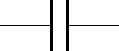
\includegraphics[width=.5\linewidth]{condens_plain}
        \end{center}
    \end{defi}
    \begin{prop}[label=prop:Ccondens]{charge et capacité}

        Quand un courant traverse le condensateur, des charges s'accumulent sur
        les plaques~: si l'une est chargée $q$, l'autre est chargée $-q$. La
        \textbf{tension à ses bornes} est \textbf{proportionnelle à $q$}, et on
        appelle ce coefficient de proportionnalité sa \textbf{capacité} notée
        $C$. On a donc
        \[\boxed{q = Cu}\]
        avec $C$ en Farad (F), $C \approx \SI{1}{\micro F}$
        \tcblower
        \begin{center}
            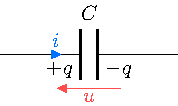
\includegraphics[width=.5\linewidth]{condens_q}
        \end{center}
    \end{prop}
\end{tcbraster}

\subsection{Caractéristique d'un condensateur}
\begin{tcbraster}[raster columns=2, raster equal height=rows]
    \begin{prop}[label=prop:Ccarac]{relation courant-tension}
        Pour un condensateur \textbf{en convention récepteur}, l'intensité que
        le traverse s'exprime par
        \[\boxed{i = C \dv{u_C}{t}}\]
    \end{prop}
    \begin{demo}[label=demo:Ccarac]{relation courant-tension}
        Par définition de $i$ et de la charge au borne de $C$,
        \begin{align*}
            i &= \dv{q}{t}\\
            i &= C \dv{u_C}{t}
        \end{align*}
    \end{demo}
    \begin{impl}[label=impl:continuité]{continuité}
        Si $u_C$ présente une variation brusque, alors $ \dv{u_C}{t}$ devrait
        être infini. Or, comme $i = C \dv{u_C}{t}$, ceci n'est pas possible
        puisque ça impliquerait que le courant le soit. Ainsi,
        \begin{framed}
            La tension $u_C(t)$ aux bornes d'un condensateur ne peut pas
            varier instantanément, c'est une fonction continue.
        \end{framed}
    \end{impl}
    \begin{impl}[label=impl:permanent]{régime permanent}
        En régime permanent (continu), les tensions et courants ne dépendent pas
        du temps. Alors $i = C \dv{u_C}{t} = 0$, ainsi
        \begin{framed}
            En régime permanent, le condensateur se comporte comme un
            interrupteur ouvert et bloque le courant.
        \end{framed}
    \end{impl}
\end{tcbraster}

\subsection{Énergie stockée dans un condensateur}
\begin{tcbraster}[raster columns=2, raster equal height=rows]
    \begin{prop}[label=prop:Ec]{énergie stockée}
        L'énergie emmagasinée dans un condensateur de tension $u_C$ est
        \begin{empheq}[box=\fbox]{equation*}
            E_C(t) = \frac{1}{2}C u_C(t)^2
        \end{empheq}
    \end{prop}
    \begin{demo}[label=demo:Ec]{énergie stockée}

        \textbf{En convention récepteur}, la puissance \textbf{reçue} est
        $\DS P_{\text{reçue}} = u_Ci = Cu_C \dv{u_C}{t} \triangleq \dv{E_C}{t}$.
        Or, $\forall f$ fonction dérivable, \fbox{$f\times f' = \left(
        \frac{1}{2}f^2 \right)'$}

        \[P_{\text{reçue}} = \dv{}{t} \left( \frac{1}{2} Cu_C{}^2 \right)
        \Rightarrow E_C(t) = \frac{1}{2}C u_C(t)^2\]
    \end{demo}
\end{tcbraster}
\begin{rema}[label=rema:genrec, sidebyside]{condensateur récepteur ou générateur}

    Par l'étude de la relation précédente, si $u_C \nearrow$, alors $\DS
    \dv{u_C}{t} > 0 \Rightarrow P_{\text{reçue}} > 0$~: ainsi, le condensateur
    reçoit bien de l'énergie au reste du circuit, et il se \textbf{comporte
    comme récepteur}.

    \tcblower

    À l'inverse, on lit que si $u_C \searrow$, alors
    $\DS \dv{u_C}{t} < 0 \Rightarrow P_{\text{reçue}} < 0$~: ainsi, le
    condensateur cède en réalité de l'énergie au reste du circuit, autrement dit
    \textbf{il peut se comporter comme générateur}~!
\end{rema}

\section{Bobine idéale}
\subsection{Présentation et caractéristique}

\begin{tcbraster}[raster columns=3, raster equal height=rows]
    \begin{defi}[label=def:bobine]{bobine}

        Une bobine est constituée de l'enroulement régulier d'une grande
        longueur d'un fil métallique, recouvert d'une gaine ou d'un vernis
        isolant. Son symbole est représenté ci-dessous.
        \tcblower
        \begin{center}
            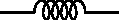
\includegraphics[width=.7\linewidth]{bobine_plain}
        \end{center}
    \end{defi}
    \begin{prop}[label=prop:Lcarac, raster multicolumn=2]{relation courant-tension}
        Quand un courant traverse la bobine, une tension apparaît à ses bornes.
        \textbf{En convention récepteur}, celle-ci s'exprime par
        \[\boxed{u_L = L\dv{i}{t}}\]
        avec $L$ l'\textbf{inductance}, exprimée en Henry (H), $L \approx
        \SI{10}{mH}$
        \tcblower
        \begin{center}
            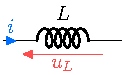
\includegraphics[width=.3\linewidth]{bobine_u}
        \end{center}
    \end{prop}
\end{tcbraster}
\begin{tcbraster}[raster columns=2, raster equal height=rows]
    \begin{impl}[label=impl:continuité]{continuité}
        Si $i$ présente une variation brusque, alors $ \dv{i}{t}$ devrait
        être infini. Or, comme $u_L = L\dv{i}{t}$, ceci n'est pas possible
        puisque ça impliquerait que la tension le soit. Ainsi,\vspace*{-10pt}
        \begin{framed}
            Le courant $i$ traversant une bobine ne peut pas
            varier instantanément, c'est une fonction continue.
        \end{framed}
    \end{impl}
    \begin{impl}[label=impl:permanent]{régime permanent}
        En régime permanent (continu), les tensions et courants ne dépendent pas
        du temps. Alors $u_L = L \dv{i}{t} = 0$, ainsi
        \begin{framed}
            En régime permanent, la bobine se comporte comme un
            fil et la tension à ses bornes est nulle
        \end{framed}
    \end{impl}
\end{tcbraster}

\subsection{Énergie stockée dans une bobine}
\begin{tcbraster}[raster columns=2, raster equal height=rows]
    \begin{prop}[label=prop:El]{énergie stockée}
        L'énergie emmagasinée dans une bobine traversée par l'intensité $i$ est
        \begin{empheq}[box=\fbox]{equation*}
            E_L(t) = \frac{1}{2}L i(t)^2
        \end{empheq}
    \end{prop}
    \begin{demo}[label=demo:Ec]{énergie stockée}

        \textbf{En convention récepteur}, la puissance \textbf{reçue} est
        $\DS P_{\text{reçue}} = u_Li = L \dv{i}{t}i \triangleq \dv{E_L}{t}$. Or,
        $\forall f$ fonction dérivable, \fbox{$f\times f' = \left(
        \frac{1}{2}f^2 \right)'$}

        \[P_{\text{reçue}} = \dv{}{t} \left( \frac{1}{2} Li^2 \right)
        \Rightarrow E_L(t) = \frac{1}{2}Li(t)^2\]
    \end{demo}
\end{tcbraster}
\begin{rema}[label=rema:genrec, sidebyside]{bobine réceptrice ou génératrice}

    Par l'étude de la relation précédente, si $i \nearrow$, alors $\DS
    \dv{i}{t} > 0 \Rightarrow P_{\text{reçue}} > 0$~: ainsi, la bobine
    reçoit bien de l'énergie au reste du circuit, et elle se \textbf{comporte
    comme un récepteur}.

    \tcblower

    À l'inverse, on lit que si $i \searrow$, alors
    $\DS \dv{i}{t} < 0 \Rightarrow P_{\text{reçue}} < 0$~: ainsi, la bobine cède
    en réalité de l'énergie au reste du circuit, autrement dit \textbf{elle peut
    se comporter comme un générateur}~!
\end{rema}

\section{Circuit RC série~: charge}

\begin{tcbraster}[raster columns=2, raster equal height=rows]
    \begin{defi}[label=def:circordre1]{circuits du premier ordre}
        On appelle \textbf{circuit linéaire du premier ordre} un circuit électrique
        dont l'évolution des grandeurs électriques est régie par des équations
        différentielles linéaires à coefficients constants et \textit{du premier
        ordre}. On étudie ici leur réponse à un échelon de tension.
    \end{defi}
    \begin{defi}[label=def:echelon, sidebyside]{échelon de tension}
        Un échelon de tension est montant s'il est de la forme
        \[ \left\{
                \begin{array}{rcl}
                    u(t<0)    & = & 0 \\
                    u(t\geq0) & = & E
                \end{array}
        \right.\]
        et descendant si $E$ avant et 0 après.
        \tcblower
        \begin{center}
            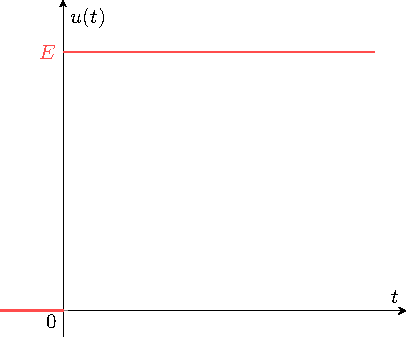
\includegraphics[width=\linewidth]{echelon}
        \end{center}
    \end{defi}
\end{tcbraster}

\subsection{Présentation}
\begin{defi}[label=def:echelonC, sidebyside]{situation initiale}
    Le montage est représenté ci-contre. Il est constitué d'un générateur idéal
    de tension en série avec une résistance et un condensateur idéal. \textbf{On
    suppose le condensateur initialement déchargé}. À $t=0$, on ferme
    l'interrupteur.
    \tcblower
    \begin{center}
        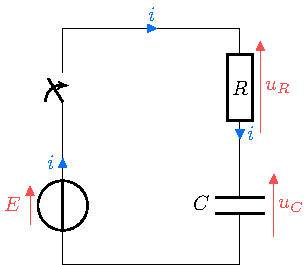
\includegraphics[width=.7\linewidth]{circ_rc-start}
    \end{center}
\end{defi}

\subsection{Équation différentielle du circuit}
\begin{tcbraster}[raster columns=2, raster equal height=rows]
    \begin{prop}[label=prop:eqdiffrc]{équation diff. RC}
        L'équation différentielle de la tension $u_C(t)$ aux bornes d'un
        condensateur dans un circuit RC avec un échelon de tension $E$
        s'écrit
        \[ \boxed{\dv{u_C}{t} + \frac{1}{\tau}u_C = \frac{E}{\tau}}\]
        avec \fbox{$\tau = RC$} la constante de temps.
        \tcblower
        C'est une équation différentielle linéaire du premier ordre à
        coefficients et second membre constants, de condition initiale
        \[ \boxed{u_C(0^-) = u_C(0^+) = 0}\]
    \end{prop}
    \begin{demo}[label=demo:eqdiffrc]{équation diff. RC}
        Avec la loi des mailles,\smallbreak
        \centersright{$u_R + u_C = E$}{(1)}\linebreak
        On utilise la loi d'Ohm et la caractéristique du condensateur~:
        $\DS u_R = Ri$ et $\DS i = C \dv{u_C}{t}$
        \begin{align*}
            (1) \Leftrightarrow RC \dv{u_C}{t} + u_C        & = E\\
            \Leftrightarrow \dv{u_C}{t} + \frac{1}{\tau}u_C & = \frac{E}{\tau}
        \end{align*}
    \end{demo}
\end{tcbraster}

\vspace{-17pt}
\subsection{Résolution de l'équation différentielle}
\begin{tcbraster}[raster columns=2, raster equal height=rows]
    \begin{tcolorbox}[blankest, raster multicolumn=1, space to=\myspace]
        \begin{tcbraster}[raster columns=1]
            \begin{prop}[label=prop:ucsolu]{solution de l'équation
                différentielle RC}
                La solution de l'équation différentielle de la tension $u_C(t)$
                d'un circuit RC soumise à un échelon de tension $E$ avec
                $u_C(0) = 0$ est
                \[\boxed{u_C(t) = E\left(1-\exp\left(-\frac{t}{\tau}\right)\right)}\]
            \end{prop}
            \begin{ror}[label=impo:eqres, heart]{résolution équation différentielle
                    coefficients constants}

                Pour résoudre une équation différentielle linéaire à
                coefficients constants et second membre constant, de la forme
                $\DS \dv{y}{y} + \frac{1}{\tau}y = k$~:
                \begin{enumerate}
                    \item On écrit l'\textbf{équation homogène} associée à
                        l'équation différentielle obtenue.
                    \item On écrit la \textbf{forme générale de la solution de
                        l'équation homogène}.
                    \item On recherche une \textbf{solution particulière
                        constante de l'équation générale}, de la forme $y(t) =
                        \lambda$.
                    \item On écrit la \textbf{solution générale}, somme de la
                        solution particulière et de la forme générale.
                    \item On détermine la constante à l'aide des
                        \textbf{conditions initiales}.
                \end{enumerate}
            \end{ror}
        \end{tcbraster}
    \end{tcolorbox}
    \begin{demo}[label=demo:rcsolu]{solution RC série}
        \begin{enumerate}
            \item L'équation homogène est~: \[ \dv{u_C}{t} + \frac{1}{\tau}u_C =
                0\]
            \item La forme générale de la solution pour cette équation est~:
                \[u_C(t) = K\exp\left( -\frac{t}{\tau} \right)\]
            \item Une solution particulière avec $u_C(t) = \lambda$ donne \[0 +
                \frac{\lambda}{\tau} = \frac{E}{\tau}\] Donc $u_C(t) = E$ est
                \textbf{une} solution de l'équation différentielle.
            \item La solution générale est donc \[ u_C(t) = E + K\exp \left( -
                \frac{t}{\tau} \right)\]

            \item Les conditions initiales donnent ici, $u_C(t=0) = 0$. Or,
                $u_C(0) = K + E$, donc $K=-E$~; ainsi
                \[\boxed{u_C(t) =
                E\left(1-\exp\left(-\frac{t}{\tau}\right)\right)}\]
        \end{enumerate}
    \end{demo}
\end{tcbraster}

\subsection{Représentation graphique et constante de temps}
\begin{tcbraster}[raster columns=2, raster equal height=rows]
    \begin{impl}[label=impl:tauRC]{constante de temps}
        \begin{center}
            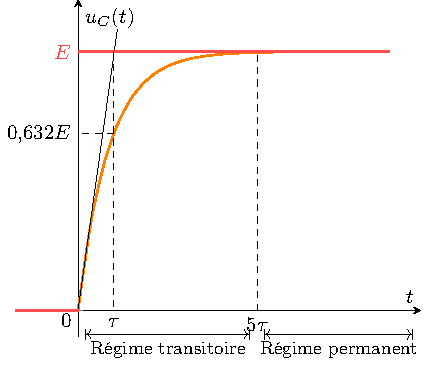
\includegraphics[width=\linewidth]{carac_rc-tau}
        \end{center}
    \end{impl}
    \begin{tcolorbox}[blankest, raster multicolumn=1]%, space to=\myspace]
        \begin{tcbraster}[raster columns=1]
            \begin{defi}[label=def:regmperma]{régime permanent}
                Le régime permanent est atteint quand $u_C(t)$ est
                suffisamment proche de l'asymptote.
            \end{defi}
            \begin{exem}[label=impl:déterm]{détermination $\tau$}
                Avec la courbe $u_C(t)$, on remarque que~:
                \begin{enumerate}
                    \item $u_C(\tau) = E \left( 1-e^{-1} \right) \approx
                        \num{0.632}\times E$~;
                    \item La tangente à la courbe en 0, de pente
                        $\dv{u}{t} (0) = \frac{E}{\tau}$, coupe l'asymptote en $t
                        = \tau$.
                \end{enumerate}
                De plus, avec $t_{99}$ tel que $u_C(t_{99}) = \num{0.99}E$, on
                trouve $t_{99} = \tau\ln(100)$~; ainsi \fbox{le temps de réponse
                à 99\% est à \num{4.6}$\tau$}.
            \end{exem}
        \end{tcbraster}
    \end{tcolorbox}
\end{tcbraster}

\subsection{Évolution de l'intensité}
\begin{tcbraster}[raster columns=2, raster equal height=rows]
    \begin{prop}[label=prop:irc-charge, sidebyside]{intensité RC charge}
        L'intensité dans un circuit RC en charge s'exprime par
        \[\boxed{i(t) = \frac{E}{R}\exp \left(-\frac{t}{\tau} \right)}\]
        \tcblower
        \begin{center}
            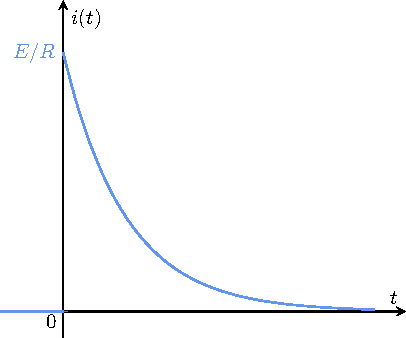
\includegraphics[width=1.1\linewidth]{carac_rcI}
        \end{center}
    \end{prop}
    \begin{demo}[label=demo:irc-charge]{intensité RC charge}
        2 méthodes~:
        \begin{enumerate}
            \item Avec la caractéristique de C
                \begin{align*}
                                i(t) &= C\DS \dv{u_C}{t}\\
                    \Rightarrow i(t) &= CE \left(0 -
                        \left(-\frac{1}{\tau} \right)
                        \exp \left(- \frac{t}{\tau} \right) \right)
                \end{align*}
                et $C/\tau = 1/R$.
            \item Avec la loi des mailles $Ri = E - u_C$. On isole $i$ en
                divisant par $R$.
        \end{enumerate}
    \end{demo}
\end{tcbraster}

\subsection{Bilan de puissance}

\begin{tcbraster}[raster columns=2, raster equal height=rows]
    \begin{prop}[label=prop:rcpuiss-charge]{bilan de puissances}
        Dans un circuit RC en charge, on a le bilan de puissances
        \[ \boxed{P_G = P_C + P_J}\]
        avec $P_G$ la puissance fournie par le générateur, $P_C = \dv{E_C}{t}$
        la puissance reçue par le condensateur et $P_J$ la puissance dissipée
        par effet Joule dans la résistance.
    \end{prop}
    \begin{demo}[label=demo:rcpuiss-charge]{bilan de puissances}
        Pour obtenir des puissances, \textbf{on écrit la loi des mailles et on
        multiplie par $i$}. Ici, $E = u_C + Ri$ multiplié par $i$ donne $Ei =
        u_Ci + Ri^2$. On a bien
        \[\boxed{P_G = Ei}, \boxed{P_C = \dv{E_C}{t}}, \boxed{P_J=Ri^2}\]
    \end{demo}
\end{tcbraster}

\subsection{Bilan d'énergie}
\begin{tcbraster}[raster columns=2, raster equal height=rows]
    \begin{prop}[label=prop:rcenerg-charge]{bilan d'énergie}
        Pendant la totalité de la charge
        $$E_G = CE^2$$
        se répartie équitablement entre le condensateur et la résistance~:
        $$E_C = \frac{1}{2} CE^2 = E_J$$
    \end{prop}
    \begin{demo}[label=demo:rcenerg-charge]{bilan d'énergie}
        L'énergie fournie par le générateur sur toute la charge est
        \begin{gather*}
            E_G = \int_{0}^{+\infty} P_G \dd t =
            \frac{E^2}{R} \left[
                -\tau \exp \left(-\frac{t}{\tau} \right)
            \right]_0^{+\infty}\\
            E_G = \tau \frac{E^2}{R} = CE^2
        \end{gather*}
        Et celle par le générateur est $E_C = \frac{1}{2}CE^2$ (propriété
        \ref{prop:Ec})~; forcément $E_J = \frac{1}{2}CE^2$.
    \end{demo}
\end{tcbraster}

\section{Circuit RC série~: décharge}
\subsection{Présentation}
\begin{defi}[label=def:echelonC, sidebyside, righthand width=.3\linewidth]
    {situation initiale}

    Le montage est représenté ci-contre. Il est constitué de l'association en
    série avec une résistance et un condensateur idéal. \textbf{On suppose le
    condensateur initialement chargé}~: $u_C(0^-) = E$. On dit que le système
    est \textbf{en régime libre} et soumis à un \textbf{échelon de tension
    descendant}

    \tcblower
    \begin{center}
        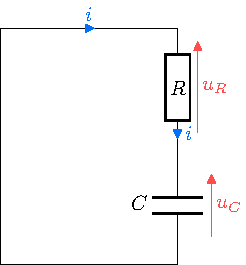
\includegraphics[width=.7\linewidth]{circ_rc-decharge}
    \end{center}
\end{defi}

\subsection{Équation différentielle du circuit}
\begin{tcbraster}[raster columns=2, raster equal height=rows]
    \begin{prop}[label=prop:eqdiffrc]{équation diff. RC}
        L'équation différentielle de la tension $u_C(t)$ aux bornes d'un
        condensateur dans un circuit RC en décharge
        \[ \boxed{\dv{u_C}{t} + \frac{1}{\tau}u_C = 0}\]
        avec \fbox{$\tau = RC$} la constante de temps.
        \tcblower
        C'est une équation différentielle linéaire du premier ordre à
        coefficients constants sans second membre, de condition initiale
        \[ \boxed{u_C(0^-) = u_C(0^+) = E}\]
    \end{prop}
    \begin{demo}[label=demo:eqdiffrc]{équation diff. RC}
        Avec la loi des mailles,
        $$u_R + u_C = 0$$
        On utilise la loi d'Ohm et la caractéristique du condensateur~:
        $\DS u_R = Ri$ et $\DS i = C \dv{u_C}{t}$
        \begin{align*}
            Ri + u_C                                        & = 0\\
            \Leftrightarrow RC \dv{u_C}{t} + u_C            & = 0\\
            \Leftrightarrow \dv{u_C}{t} + \frac{1}{\tau}u_C & = 0
        \end{align*}
    \end{demo}
\end{tcbraster}

\subsection{Résolution de l'équation différentielle}
\begin{tcbraster}[raster columns=2, raster equal height=rows]
    \begin{prop}[label=prop:ucsolu]{solution de l'équation
        différentielle RC}
        La solution de l'équation différentielle de la tension $u_C(t)$
        d'un circuit RC en décharge avec $u_C(0) = E$ est
        \[\boxed{u_C(t) = E\exp\left(-\frac{t}{\tau}\right)}\]
    \end{prop}
    \begin{demo}[label=demo:rcsolu]{solution RC série}
        L'équation étant déjà homogène, on écrit la forme générale~:
        \[u_C(t) = K\exp\left( -\frac{t}{\tau} \right)\]
        et on trouve $K$ avec la condition initiale~: $u_C(t=0) = E$. Or,
        $u_C(0) = K$, donc $K=E$, d'où la réponse demandée.
    \end{demo}
\end{tcbraster}

\subsection{Représentation graphique et constante de temps}
\begin{tcbraster}[raster columns=2, raster equal height=rows]
    \begin{impl}[label=impl:tauRC]{constante de temps}
        \begin{center}
            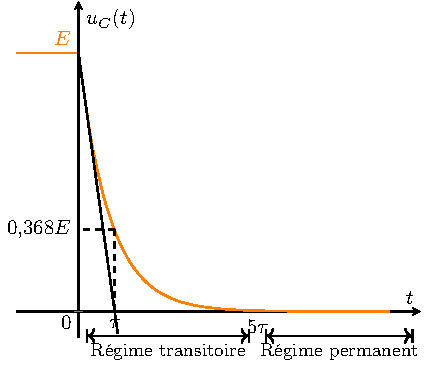
\includegraphics[width=\linewidth]{carac_rc-tau_decharge}
        \end{center}
    \end{impl}
    \begin{exem}[label=impl:déterm]{détermination $\tau$}
        Avec la courbe $u_C(t)$, on remarque que~:
        \begin{enumerate}
            \item $u_C(\tau) = E e^{-1} \approx \num{0.368}\times E$~;
            \item La tangente à la courbe en 0, de pente $- \frac{E}{\tau}$,
                coupe l'asymptote en $t = \tau$.
        \end{enumerate}
        Comme précédemment, avec $t_{99}$ tel que $u_C(t_{99}) = \num{0.01}$, on
        trouve $t_{99} = \num{4.6}\tau$.
    \end{exem}
\end{tcbraster}

\subsection{Évolution de l'intensité}

\begin{tcbraster}[raster columns=2, raster equal height=rows]
    \begin{prop}[label=prop:irc-charge, sidebyside,
        righthand width=.15\linewidth]{intensité RC charge}
        L'intensité dans un circuit RC en décharge s'exprime par
        \[\boxed{i(t) = -\frac{E}{R}\exp \left(-\frac{t}{\tau} \right)}\]
        \tcblower
        \hspace*{-12pt}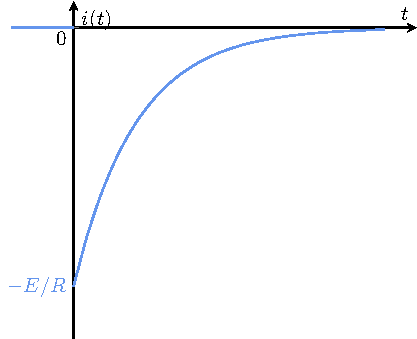
\includegraphics[width=1.3\linewidth]{carac_rcI-decharge}
    \end{prop}
    \begin{demo}[label=demo:irc-charge]{intensité RC charge}
        2 méthodes~:
        \begin{enumerate}
            \item Avec la caractéristique de C
                \begin{align*}
                                i(t) &= C\DS \dv{u_C}{t}\\
                    \Rightarrow i(t) &= - \frac{CE}{\tau} \exp \left(-
                    \frac{t}{\tau} \right)
                \end{align*}
                et $C/\tau = 1/R$.
            \item Avec la loi des mailles $Ri = -u_C$. On isole $i$ en
                divisant par $R$.
        \end{enumerate}
    \end{demo}
\end{tcbraster}

\section{Circuit RL série~: échelon montant}
\subsection{Présentation}
\begin{defi}[label=def:echelonL, sidebyside]{situation initiale}
    Le montage est représenté ci-contre. Il est constitué d'un générateur idéal
    de tension en série avec une résistance et une bobine idéale. À $t=0$, on
    ferme l'interrupteur et le circuit est donc soumis à un échelon de tension
    montant.
    \tcblower
    \begin{center}
        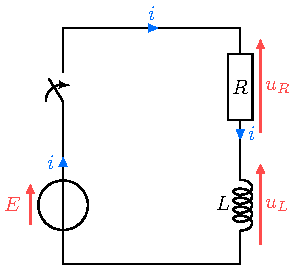
\includegraphics[width=.7\linewidth]{circ_rl-start}
    \end{center}
\end{defi}

\subsection{Équation différentielle du circuit}
\begin{tcbraster}[raster columns=2, raster equal height=rows]
    \begin{prop}[label=prop:eqdiffrc]{équation diff. RL}
        L'équation différentielle de l'intensité $i(t)$ traversant la bobine
        dans un circuit RL avec un échelon de tension $E$ s'écrit
        \[ \boxed{\dv{i}{t} + \frac{1}{\tau}i = \frac{E}{R\tau}}\]
        avec \fbox{$\tau = L/R$} la constante de temps.
        \tcblower
        C'est une équation différentielle linéaire du premier ordre à
        coefficients et second membre constants, de condition initiale
        \[ \boxed{i(0^-) = i(0^+) = 0}\]
    \end{prop}
    \begin{demo}[label=demo:eqdiffrc]{équation diff. RL}
        Avec la loi des mailles,\smallbreak
        \centersright{$u_L + u_C = E$}{(1)}\linebreak
        On utilise la loi d'Ohm et la caractéristique de la bobine~:
        $\DS u_R = Ri$ et $\DS u_L = L \dv{i}{t}$
        \begin{align*}
            (1) \Leftrightarrow L\dv{i}{t} + Ri         & = E\\
            \Leftrightarrow \dv{i}{t} + \frac{1}{\tau}i & = \frac{E}{R\tau}
        \end{align*}
    \end{demo}
\end{tcbraster}

\subsection{Résolution de l'équation différentielle}
\begin{tcbraster}[raster columns=2, raster equal height=rows]
    \begin{prop}[label=prop:ucsolu]{solution de l'équation
        différentielle RL}
        La solution de l'équation différentielle du courant $i(t)$
        d'un circuit RL soumis à un échelon de tension $E$ avec
        $i(0) = 0$ est
        \[\boxed{i(t) = \frac{E}{R}\left(1-\exp\left(-\frac{t}{\tau}\right)\right)}\]
    \end{prop}
    \begin{demo}[label=demo:rcsolu]{solution RC série}
        L'équation homogène $\DS\dv{i}{t} + \frac{1}{\tau}i = 0$ a pour forme
        générale de solution $i(t) = K\exp\left( -\frac{t}{\tau}
        \right)$.\smallbreak
        $i(t) = \lambda$ $\Leftrightarrow\DS0 + \frac{\lambda}{\tau} =
        \frac{E}{R\tau}$, soit $\lambda = \frac{E}{R}$.\smallbreak
        Ainsi, la solution générale est $i(t) = \frac{E}{R} + K\exp
        \left(-\frac{t}{\tau} \right)$. Avec $i(0) = 0$, on trouve $K = -E/R$,
        d'où finalement la solution.
    \end{demo}
\end{tcbraster}

\subsection{Représentation graphique et constante de temps}
\begin{tcbraster}[raster columns=2, raster equal height=rows]
    \begin{impl}[label=impl:tauRC]{constante de temps}
        \begin{center}
            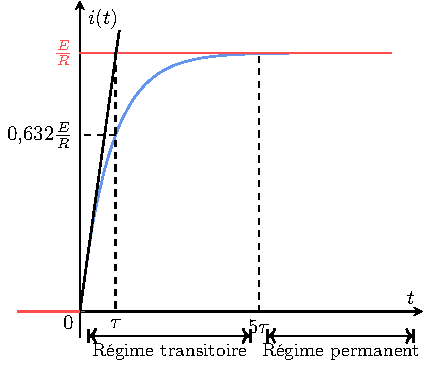
\includegraphics[width=\linewidth]{carac_rl-tau}
        \end{center}
    \end{impl}
    \begin{tcolorbox}[blankest, raster multicolumn=1]%, space to=\myspace]
        \begin{tcbraster}[raster columns=1]
            \begin{defi}[label=def:regmperma]{régime permanent}
                Le régime permanent est atteint quand $i(t)$ est
                suffisamment proche de l'asymptote.
            \end{defi}
            \begin{exem}[label=impl:déterm]{détermination $\tau$}
                Avec la courbe $i(t)$, on remarque que~:
                \begin{enumerate}
                    \item $i(\tau) = \frac{E}{R} \left( 1-e^{-1} \right) \approx
                        \num{0.632}\times \frac{E}{R}$~;
                    \item La tangente à la courbe en 0, de pente $
                        \frac{E}{R\tau}$ coupe l'asymptote en $t = \tau$.
                \end{enumerate}
                De plus, avec $t_{99}$ tel que $i(t_{99}) =
                \num{0.99}\frac{E}{R}$, on trouve $t_{99} = \tau\ln(100)$~;
                ainsi \fbox{le temps de réponse à 99\% est à \num{4.6}$\tau$}.
            \end{exem}
        \end{tcbraster}
    \end{tcolorbox}
\end{tcbraster}

\subsection{Évolution de la tension}
\begin{tcbraster}[raster columns=2, raster equal height=rows]
    \begin{prop}[label=prop:irc-charge, sidebyside, righthand ratio=.45]{tension RL}
        La tension dans un circuit RL s'exprime par
        \[\boxed{u_L(t) = E\exp \left(-\frac{t}{\tau} \right)}\]
        \tcblower
        \begin{center}
            \hspace*{-12pt}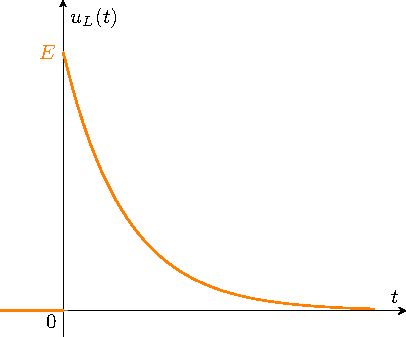
\includegraphics[width=1.3\linewidth]{carac_rlU}
        \end{center}
    \end{prop}
    \begin{demo}[label=demo:irc-charge]{intensité RC charge}
        2 méthodes~:
        \begin{enumerate}
            \item Avec la caractéristique de L
                \begin{align*}
                                u_L(t) &= L\DS \dv{i}{t}\\
                    \Rightarrow u_L(t) &= \frac{LE}{R} \left(0 -
                        \left(-\frac{1}{\tau} \right)
                        \exp \left(- \frac{t}{\tau} \right) \right)
                \end{align*}
                et $\tau = L/R$.
            \item Avec la loi des mailles $u_L = E - Ri$.
        \end{enumerate}
    \end{demo}
\end{tcbraster}

\subsection{Bilan de puissance}

\begin{tcbraster}[raster columns=2, raster equal height=rows]
    \begin{prop}[label=prop:rcpuiss-charge]{bilan de puissances}
        Dans un circuit RC en charge, on a le bilan de puissances
        \[ \boxed{P_G = P_L + P_J}\]
        avec $P_G$ la puissance fournie par le générateur, $P_L = \dv{E_L}{t}$
        la puissance reçue par le condensateur et $P_J$ la puissance dissipée
        par effet Joule dans la résistance.
    \end{prop}
    \begin{demo}[label=demo:rcpuiss-charge]{bilan de puissances}
        Pour obtenir des puissances, \textbf{on écrit la loi des mailles et on
        multiplie par $i$}. Ici, $E = u_L + Ri$ multiplié par $i$ donne $Ei =
        u_Li + Ri^2$. On a bien (cf.\ énergie stockée)
        \[\boxed{P_G = Ei}, \boxed{P_L = \dv{E_L}{t}}, \boxed{P_J=Ri^2}\]
    \end{demo}
\end{tcbraster}
\textbf{Ici la puissance en régime permanent n'est pas nulle~: un courant circule
toujours dans la résistance qui dissipe $RI^2$. On ne peut intégrer à l'infini.}

\section{Circuit RL série~: décharge}
\subsection{Présentation}
\begin{defi}[label=def:dechL, sidebyside, righthand width=.3\linewidth]
    {situation initiale}

    Le montage est représenté ci-contre. Il est constitué de l'association en
    série avec une résistance et une bobine idéale. À $t = 0$ on coupe la
    tension $E$ présente initialement, et le circuit est donc soumis à un
    échelon de tension descendant, et donc en régime libre.

    \tcblower
    \begin{center}
        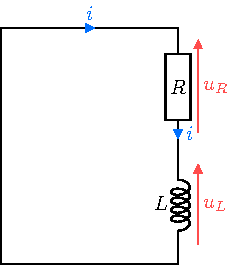
\includegraphics[width=.7\linewidth]{circ_rl-decharge}
    \end{center}
\end{defi}

\subsection{Équation différentielle du circuit}
\begin{tcbraster}[raster columns=2, raster equal height=rows]
    \begin{prop}[label=prop:eqdiffrldech]{équation diff. RL libre}
        L'équation différentielle de l'intensité $i(t)$ traversant une bobine
        dans un circuit RL en décharge est
        \[ \boxed{\dv{i}{t} + \frac{1}{\tau}i = 0}\]
        avec \fbox{$\tau = L/R$} la constante de temps.
        \tcblower
        C'est une équation différentielle linéaire du premier ordre à
        coefficients constants sans second membre, de condition initiale
        \[ \boxed{i(0^-) = i(0^+) = \frac{E}{R}}\]
    \end{prop}
    \begin{demo}[label=demo:eqdiffrc]{équation diff. RC}
        Avec la loi des mailles,
        $$u_L + u_R = 0$$
        On utilise la loi d'Ohm et la caractéristique de la bobine~:
        $\DS u_R = Ri$ et $\DS u_L = L \dv{i}{t}$
        \begin{align*}
            \Leftrightarrow L\dv{i}{t} + Ri             & = 0\\
            \Leftrightarrow \dv{i}{t} + \frac{1}{\tau}i & = 0
        \end{align*}
    \end{demo}
\end{tcbraster}

\subsection{Résolution de l'équation différentielle}
\begin{tcbraster}[raster columns=2, raster equal height=rows]
    \begin{prop}[label=prop:ulsoludech]{solution de l'équation
        différentielle RL}
        La solution de l'équation différentielle de la tension $i(t)$
        d'un circuit RL en décharge avec $i(0) = \frac{E}{R}$ est
        \[\boxed{i(t) = \frac{E}{R}\exp\left(-\frac{t}{\tau}\right)}\]
    \end{prop}
    \begin{demo}[label=demo:rcsolu]{solution RC série}
        L'équation étant déjà homogène, on écrit la forme générale~:
        \[i(t) = K\exp\left( -\frac{t}{\tau} \right)\]
        et on trouve $K$ avec la condition initiale~: $i(t=0) = \frac{E}{R}$.
        Or, $i(0) = K$, donc $K= \frac{E}{R}$, d'où la réponse demandée.
    \end{demo}
\end{tcbraster}

\subsection{Représentation graphique et constante de temps}
\begin{tcbraster}[raster columns=2, raster equal height=rows]
    \begin{impl}[label=impl:tauRC]{constante de temps}
        \begin{center}
            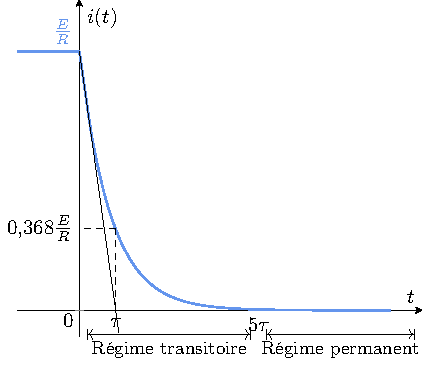
\includegraphics[width=\linewidth]{carac_rl-tau_decharge}
        \end{center}
    \end{impl}
    \begin{exem}[label=impl:déterm]{détermination $\tau$}
        Avec la courbe $i(t)$, on remarque que~:
        \begin{enumerate}
            \item $i(\tau) = \frac{E}{R} e^{-1} \approx \num{0.368}\times
                \frac{E}{R}$~;
            \item La tangente à la courbe en 0, de pente $-\frac{E}{R\tau}$,
                coupe l'asymptote en $t = \tau$.
        \end{enumerate}
        Comme précédemment, avec $t_{99}$ tel que $i(t_{99}) = \num{0.01}$, on
        trouve $t_{99} = \num{4.6}\tau$.
    \end{exem}
\end{tcbraster}

\subsection{Évolution de la tension}

\begin{tcbraster}[raster columns=2, raster equal height=rows]
    \begin{prop}[label=prop:irc-charge, sidebyside,
        righthand width=.15\linewidth]{tension RL libre}
        La tension dans un circuit RL libre s'exprime par
        \[\boxed{u_L(t) = -E\exp \left(-\frac{t}{\tau} \right)}\]
        \tcblower
        \hspace*{-12pt}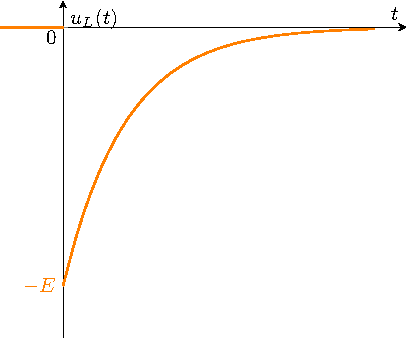
\includegraphics[width=1.3\linewidth]{carac_rlU_decharge}
    \end{prop}
    \begin{demo}[label=demo:url-decharge]{tension RL libre}
        2 méthodes~:
        \begin{enumerate}
            \item Avec la caractéristique de L
                \begin{align*}
                                u_L(t) &= L\DS \dv{i}{t}\\
                    \Rightarrow u_L(t) &= - \frac{LE}{R\tau} \exp \left(-
                    \frac{t}{\tau} \right)
                \end{align*}
                et $\tau = L/R$.
            \item Avec la loi des mailles $u_L = -Ri$.
        \end{enumerate}
    \end{demo}
\end{tcbraster}

\end{document}
